\chapter{Integration of Transcriptomic with Proteomic data}\label{ch:Integration}
After assessing the similarity of the human gene expression profiles
across various tissues
at transcriptomic level (with \Rnaseq\ studies in \Cref{ch:Transcriptomics})
and proteomic level (with \emph{bottom-up} \ms\ studies in \Cref{ch:proteomics}),
my next step is to examine how these gene expression profiles
compare between these two different biological layers.

One major aim of this study is to asses
how the correlations between the transcriptome and proteome
described in the literature, mostly measured in cells,
hold at the tissue level.
Moreover, good correlations may potentially lead to
the development of new strategies.
These may use the expression levels of \mRNA\ as proxies
to estimate protein expression,
which is generally difficult to measure directly (see \Cref{sec:exploreProtMS}).

I have performed the integration and all the analyses presented in this chapter
under the supervision of \alvis\ and \jyoti.
A manuscript describing this work
and the new method of protein quantification, presented in \Cref{sec:NewQuantProt},
is being prepared.

A few closely related studies~\mycite{SciRep2016,Franks2017-bp} have
been published while I was working on
the integration of the non-diseased human transcriptome and proteome.
As their analyses rely on the same data sets (\ie\ \uhlen, \gtex, \pandey\ data)
that I include in my work,
I describe and discuss together my results and theirs
whenever relevant.

\derivativeWork{}
\begin{itemize}[topsep=0pt,nosep]
    \item (poster) CSHL  Biology of Genomes 2015 --- A feasibility study:
        Integration of independent human \Rnaseq\ and proteomic datasets
\end{itemize}

\clearpage\

\vspace{-1cm}

One on-going debate in the literature is
whether good correlations of expression levels should prevail or not
between matching \mRNAs\ and proteins \mycite{Uhlen:2016}.
The implicit assumption of a proportional relationship is persisting
because of the many remaining technological limitations \mycite{Vogel2012-sq},
whereas to date, the existence of a given \mRNA\ transcript or its concentration
are usually insufficient to ensure detection of the protein in a sample.

On the one hand,
\citet{Ramakrishnan2009-lv} report that
\mRNAs\ abundance are roughly sufficient to predict
the protein presence or absence from a sample and
\citet{Vogel2010-ux} that
\mRNA\ level estimations and sequence features are enough to predict
two-thirds of the human protein abundance variation.\\
\vspace{-\baselineskip}

On the other hand,
there is a lack of high correlations
between the transcriptome and proteome
(for any organism) observation in the literature.
Previous investigations found low or no correlation
between the observed expression profiles of the \mRNAs\ and
proteins~\mycite{Anderson1997-le,Chen2002-ob,Tian2004-hh,Pascal2008-gh,%
Gry2009-zv,Lundberg2010-gk}.
This observation lack is unrestricted to human \mycite{Ghazalpour2011-nb} or
even mammals~\mycite{Gygi1999-fl,Maier2009-pb,Maier2011-tz,Yeung2011-sl,%
Palmblad2013-ji,Freiberg2016-fu}.\\
\vspace{-\baselineskip}

Additionally,
Schwanhäusser et al.~\mycite{schwanhausserglobal:2011,Schwanhausser2013-et}
present rather moderate correlations ($r^2≤0.41,\ie~r<0.64$)
for their encompassing experiment
and highlight that \mRNAs\ levels explain only about 40\% of protein variations
they have observed.

Other studies tried to explore the \mRNAs\ and proteins relationship in answer
to stimuli.
\citet{Marguerat2012-sn} report for yeast that
steady-state cells present an equivalent level of correlation ($r^2=0.36,
\ie~r=0.6$) to the previous studies,
while proliferating cells present higher correlations ($r^2=0.55, \ie~r=0.74$).
\citet{Jovanovic2015-wv} identify \mRNA\ fold changes
as the most prominent contributor to the relative changes in protein expression
for 89\% of the mouse immune genes of their study,
before concluding that relative changes in \mRNAs\ levels can explain
\emph{relative} changes in protein levels,
while post-transcriptional regulations (including degradation rates)
better explain the \emph{absolute} amount of proteins.

While many other regulations processes may occur,
post-transcriptional modifications and technical noise
are (still) perceived as the probable primary sources
of \mRNA/protein concentration discrepancies~\mycite{Vogel2012-sq,Plotkin2010-ug}.
Although
the joint study of transcriptome and proteome has already helped to highlight
links between genotype and phenotype~\mycite{Vogel2012-sq},
the previous mitigated results probably explain the focus shift of
many subsequent studies.
Previous efforts were about linking the actual expression levels.
More recent studies primarily compare qualitative attributes
of given proteins and related \mRNAs,
such as their presence or absence in a specific condition
or tissue~\mycite{Santos2015-rj,Freiberg2016-fu,Uhlen2015}
or their differential expression profiles across the same set of conditions
to detect any discrepancy~\mycite{Varemo2015-uk}.

All (or almost all) aforementioned studies have all turned to cells
for their joint analyses of transcriptome and proteome.
The analyses and integration I present in this chapter are
on the other hand based on tissue studies.

\vspace{-2mm}
\section{Data~and~principal~analytical~approaches}\label{sec:IntegrationData}
\vspace{-4mm}
Since 2014 and the human proteome drafts \mycite{PandeyData,KusterData},
this is the first time with such
an unparalleled availability of large-scale tissue studies
both at the transcriptomic and proteomic layers to explore and integrate together
(see \Cref{ch:datasets}).
While these data are independent
(collected from various individuals, prepared,
and characterised by different laboratories),
their combined study may help
to shed light on the relationship
between the transcriptome and proteome at the tissue level.
Using different sources for the transcriptome and proteome
increases the overall technical noise,
but it may also help to highlight relevant biological signals (as
they need to be stronger than the noise and batch effects to be captured).

In \Cref{ch:Transcriptomics}, I show that
the transcriptome \Rnaseq\ datasets present high correlations
(median value for Pearson: $r_{\setOneMath}=0.75$; $r_{\setTwoMath}=0.85$ ---
Spearman: $\rho_{\setOneMath}=0.88$; $\rho_{\setTwoMath}=0.93$).
For this chapter analyses,
I only consider the datasets with the highest similarity
(highest correlations) and
that incidentally comprise the greatest number of tissues
and are the two most recent studies,
\ie\ \dataset{Uhlén \etal}~\mycite{Uhlen2015}
and \dataset{Gtex}~\mycite{GTExTranscript} data.\\
\vspace{-\baselineskip}

Since I am reusing published data,
the initial experimental designs are suboptimal for my study.
Using both \uhlen\ and \gtex\ data
allows filtering out \mRNAs\ with high variability.
Whether this variability is technical or biological is irrelevant;
in both cases,
interpreting the relationship
between a highly variable \mRNAs\ and its protein from another dataset
remains hard to interpret.
Besides, the comparison of the two transcriptomic data may give a reference,
\ie\ an ideal case scenario, for the proteomic/transcriptomic one.

On the other hand,
the technical variability prevails over
the biological signal of same-tissue samples
for the available high-throughput proteomics,
as shown in \Cref{subsec:protTechVarHigh}.
To avoid an overly restricted protein set for the following analyses,
I only include one proteomic study: \pandey\ et al.~\mycite{PandeyData}.
All its samples have been run through the same \ms\ platform and
with the same protocol.
Besides, it presents more homogeneous protein distributions
(see \Cref{fig:distribProt} and \Cref{fig:pandeyDistribQ1Q2}) and
quantifies more proteins per tissues (\Cref{fig:distribProtUniq3D})
than the two other datasets.
As one of the main current limitations of bottom-up \ms\ proteomic studies
is the possible lack of detection of proteins for various reasons
(see \Cref{subsec:simpleProt}),
it suggests that
the \pandey\ data has a higher quality than the two other datasets.

%Many strategies are recommended to increase the depth of the coverage
%(\eg\ \mycite{Zhang2014,Eriksson2007-si,Koziol2013-si}).
%Put together these facts suggest that
%the \pandey\ data has a higher quality than the two other datasets.
\vspace{-0.5mm}
As the literature reports that
the proteome is more conserved than the transcriptome
(across individuals and species)~\mycite{Laurent2010-rg,Liu2016-re},
this data collection ought to provide
a crude estimate of the extent of observations
that hold from cell to tissue level.

This chapter integrates and analyses the matching pairs of \mRNA/proteins
of the common set of tissues between \pandey\ \etal\
and the two transcriptomic datasets.

\vspace{-2.5mm}
\subsection{Overlapping set of tissues for the three datasets}

\begin{figure}[!htbp]
    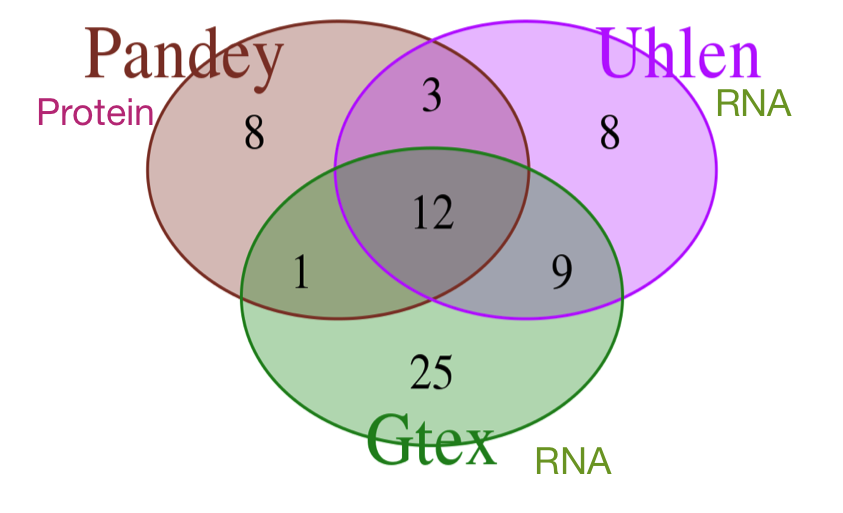
\includegraphics[scale=0.61]{integration/PandeyGtexUhlen_tissuesVenn.pdf}
    \centering
    \vspace{-5mm}
    \caption[Number of shared and unique tissues between the proteomic
    dataset from Pandey \etal\ and the transcriptomic datasets (Uhlén \etal\ and
    Gtex)]{\label{fig:VennTissuePandeyGtexUhlen}\textbf{Number of shared and unique
    tissues between the proteomic (Pandey \etal) and the
    transcriptomic (Uhlén \etal\ and GTEx) data.} The twelve common tissues of
    the three datasets are
    \tissue{Adrenal gland}, \tissue{Bladder}, \tissue{Colon}, \tissue{Oesophagus},
    \tissue{Heart}, \tissue{Kidney}, \tissue{Liver}, \tissue{Lung}, \tissue{Ovary},
    \tissue{Pancreas}, \tissue{Prostate} and \tissue{Testis}. The three added
    tissue between \dataset{Uhlén \etal} and \dataset{Pandey \etal} are
    \tissue{Gall bladder}, \tissue{Placenta} and \tissue{Rectum}. The added tissue
    between \dataset{GTEx} and \dataset{Pandey \etal} is the \tissue{Frontal
    cortex}.}
\end{figure}

All the analyses are including the twelve shared tissues between the three
datasets (\adrenal, \Bladder{}\footnote{May also
be referred as \tissue{Urinary Bladder}},
\hColon, \Oesophagus, \Heart,
\Kidney, \Liver, \Lung, \Ovary, \Pancreas,
\Prostate\ and \Testis).

\vspace{-1.5mm}
In a few cases, I have also extended the analyses by excluding the \gtex\ data
to include the three added tissues shared by
\pandey\ et al.\ and \uhlen\ et al.\ data (\ie\ \Gall, \Placenta\ and \Rectum).

\vspace{-2mm}
\subsection{Matching pairs of mRNAs and proteins}

\vspace{-3mm}
As formerly described in \Cref{sec:bias_sources},
to avoid unnecessary biases I only consider for the following analyses
\mRNAs\ (\ie\ \glspl{RNA} with a \emph{protein-coding} biotype --- \ens{76})
and proteins that are found in each dataset at least in one of the included tissues.

Besides, while there is only one value per protein per tissue,
both \uhlen\ \etal\ and \gtex\ data present replicates,
\ie\ there are several values per \mRNA\ per tissue
for each of the transcriptomic datasets.
Thus, I use the \enquote{virtual references},
\ie\ \treps\footnote{\trep{}: \glsdesc{TREP}}
that I describe in \Cref{subsec:averagedTissue},
to avoid unbalancing the analyses.\\
\vspace{-\baselineskip}

\Cref{fig:PGU_vennQ1} presents the matches between
the proteins from the \pandey\ \etal\ data
quantified through the pipeline described in \Cref{subsec:msDataProcess}
and the \mRNAs\ of \uhlen\ \etal\ and \gtex\ data quantified by \htseq\
(see \Cref{subsubsec:RnaseqDataProc}) across their twelve common tissues.

\begin{figure}[!htb]
    \includegraphics[scale=0.65]{integration/PandeyGtexUhlen_mRNAprotQ1Venn.pdf}\centering
    \vspace{-5mm}
    \caption[Distribution of the unique and shared proteins/mRNAs for the three datasets
    across twelve tissues]{%
    \label{fig:PGU_vennQ1}\textbf{Distribution of the unique and shared proteins
    of Pandey et al.\ data and mRNAs from Uhlén et al.\ and GTEx ones across
    their twelve shared tissues.}
    There are 6,357 matching gene products between the three datasets.
    Only 5 proteins have apparently no matching partners
    in the \uhlen\ \etal\ or \gtex\ data.}
\end{figure}

\Cref{fig:PU_vennQ1} is a replication of the previous \Cref{fig:PGU_vennQ1}
based on the removal of the \gtex\ data
and the addition of the three supplementary tissues solely shared
by \pandey\ \etal\ et \uhlen\ \etal\ data.%\\
%\vspace{-\baselineskip}

\begin{figure}[!htb]
    \includegraphics[scale=0.65]{integration/PandeyUhlen_mRNAprotQ1Venn.pdf}\centering
    \vspace{-3.5mm}
    \caption[Distribution of the unique and shared proteins/mRNAs for Pandey et al.\
    and Uhlén et al.\ across fifteen tissues.]{%
    \label{fig:PU_vennQ1}\textbf{Distribution of the unique and shared proteins/mRNAs
    for Pandey et al.\ and Uhlén et al.\ across their fifteen shared tissues.}
    The number of matching pairs (6,428) and proteins that lack a counterpart in
    the transcriptomic data (8) are similar regardless of how many different
    transcriptomic data is included (see \Cref{fig:PGU_vennQ1}).}
\end{figure}

Both figures show that almost all proteins are matching an \mRNA{},
although only about 32\% of the quantified \mRNAs\
in the \uhlen\ \etal\ and \gtex\ data
have a corresponding protein in the \pandey\ \etal\ data.

The protein quantification (provided by \james) follows
a state-of-the-art protocol and very stringent parameters
since accurate protein quantification is paramount for reliable proteome exploration.

However, I aim to integrate proteomic data with transcriptomics.
Hence, more flexible protein identification and quantification methods are possible.
Therefore, for this chapter analyses and integration,
I have devised a new quantification method that \james\ has implemented.%\\
%\vspace{-\baselineskip}

This new method emulates an \Rnaseq\ quantification approach
as I describe in \Cref{sec:NewQuantProt}.
It takes advantage of the \emph{degenerate} peptides
and allows the quantification of proteins even matched by two unique peptides only.\\
\vspace{-\baselineskip}

\begin{figure}[!ht]
    \includegraphics[scale=0.62]{integration/PandeyGtexUhlen_mRNAprotQ3Venn.pdf}\centering
    \vspace{-4mm}
    \caption[Distribution of the unique and shared proteins/mRNAs
    across the three datasets and twelve tissues
    (with the new protein quantification method)]{\label{fig:PGU_venQ3}%
    \textbf{Distribution of the unique and shared proteins/mRNAs
    across the Pandey et al.\ (processed with the new quantification method),
    Uhlén et al.\ and GTEx data across their twelve shared tissues}.
    }
\end{figure}

\begin{figure}[!ht]
    \includegraphics[scale=0.62]{integration/PandeyUhlen_mRNAprotQ3Venn.pdf}\centering
    \vspace{-4mm}
    \caption[Distribution of the unique and shared proteins/mRNAs for the
    Pandey et al.\ (processed with the new quantification method) and Uhlén et al.\ data
    across the fifteen tissues.
    ]{\label{fig:PU_vennQ3}\textbf{Distribution of the
    unique and shared proteins/mRNAs} for
    the Pandey et al.\ (processed with the new quantification method)
    and Uhlén et al.\ data across the fifteen tissues.}
\end{figure}

\Cref{fig:PGU_venQ3,fig:PU_vennQ3} are
the counterparts of \Cref{fig:PGU_vennQ1,fig:PU_vennQ1}.
With the new quantification method for the \pandey\ \etal\ data,
although the number of unmatched proteins remains marginal,
about 62\% of \uhlen\ \etal{}'s and \gtex{}'s quantified \mRNAs\
are matched to a protein.

I exclude the unmatched proteins and \mRNAs\ from further analyses.
\Cref{tab:protNoTrans} provides the unmatched protein lists
for the \ens{76} annotation.\\
\vspace{-\baselineskip}

Whether or not it reflects the biological reality,
current technology detects more individual \mRNAs\ than proteins
as confirmed by \Cref{fig:UniqExprPC1,fig:distribProtUniq3D}.
Thus, it may be primarily surprising that
a few proteins lack a match in the transcriptome data.
Several possible explanations exist.

Artefacts or technical issues are the most likely.
For example, the annotation of the matching \RNA\ is missing
or is defined with another biotype than \emph{protein-coding}.
Or, peptides and \mRNA\ reads may be assigned to different gene IDs.
Alternatively, the \mRNAs\ are present in the sample,
but the library preparation has missed their capture
(see \Cref{subsec:libPrep}).
Or even, the presence of proteins in the sample is a false positive
or the result of contamination.

However, an underlying biological phenomenon also stands as a possibility.
For example, the \mRNAs\ have a very low turnover while the proteins are very stable.
Alternatively, the proteins are expressed elsewhere before being imported in the studied tissue
(\eg\ hormones or cytokines).

Lastly, as the transcriptomic and proteomic samples are independently sourced,
a protein may be specific to an individual or a population.
This last hypothesis is the most unlikely
as there are several biological replicates on the transcriptomic side.
A mixture of the previous causes is highly probable.

Unless otherwise stated, to avoid the issues exposed in \Cref{subsec:mito},
I also remove all the proteins and \mRNAs\ of the mitochondrial genome
from the subsequent analyses.

\vspace{-3mm}
\subsection{Tissue-centric and gene-centric approaches}
\vspace{-3mm}
\begin{figure}[!htb]
    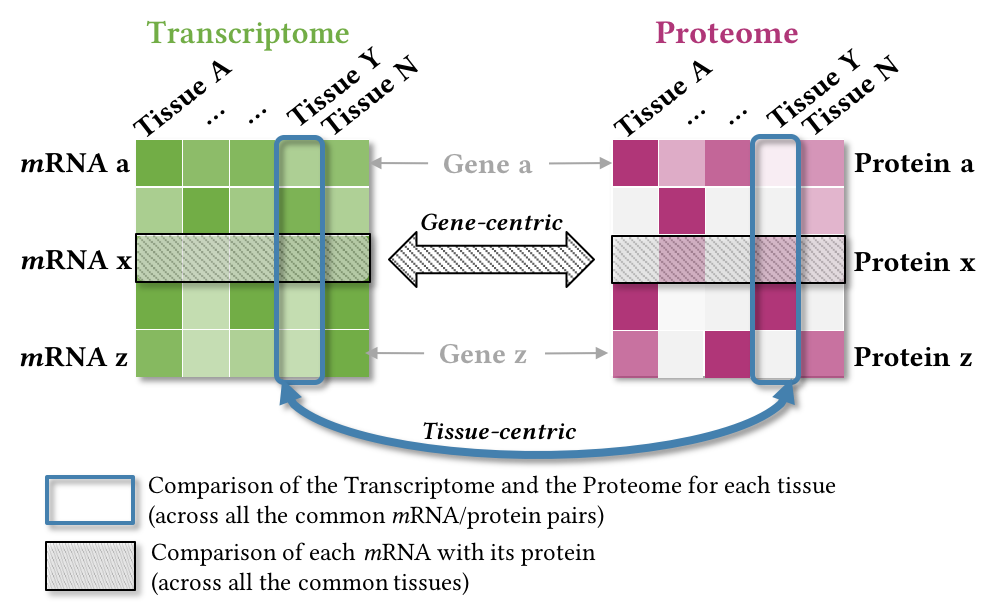
\includegraphics[scale=0.85]{integration/VisualExplaination-Lin.png}\centering
    \vspace{-3mm}
    \caption[Summary of the expression comparison approaches between
    the transcriptome and proteome]{\label{fig:visualexp}\textbf{Approaches
    summary of the expression comparison between the transcriptome and proteome.}
    \emph{Tissue-centric} analyses focus on
    how the transcriptome and proteome relate to each other within the same tissue.
    \emph{Gene-centric} analyses study for each gene how its \mRNA\ expression
    levels across all (or a subset of) the tissues may relate to
    the quantified expression levels of its corresponding protein.
    }
\end{figure}

\Cref{fig:visualexp} summarises the two analytical approaches I use
to compare transcriptomic and proteomic data.
The \emph{tissue-centric} approach compares for each tissue
the global expression of its transcriptomic landscape to its proteomic one.
In contrast,
the \emph{gene-centric} approach compares for each gene
the expression levels of its \mRNA\ to its protein ones across all the tissues.

\sectionmark{Fair correlations between independent proteomics and transcriptomics}
Although not explicitly indicated,
I use both tissue-centric and gene-centric approaches
in \Cref{ch:Transcriptomics,ch:proteomics}.
The \mRNAs\ studies are equivalent enough and
the proteomic studies so disparate that
global understanding remains unaffected without any precision.

On the other hand, many confusions can arise
when integrating proteomics and transcriptomics.
Hence, it is essential
to define the approach for this latter case clearly \mycite{Liu2016-re}.

\section{Fair correlations between independently sourced proteomics~%
and~transcriptomics~of~human~tissues~}\label{subsec:IntegrationGoodCorrProtTrans}
\sectionmark{Fair correlations between independent proteomics and transcriptomics}

As the first tissue-centric analysis,
I assess for each tissue the relationship between
the expression of its proteome and transcriptome
through the correlation of the protein expression values
with their corresponding \mRNA\ ones.\\
\vspace{-\baselineskip}

As illustrated by \Cref{fig:distribTrans,fig:pandeyDistribQ1Q2},
the proteomic and transcriptomic \treps\ expression profiles are similar
in shape at a logarithmic scale
and roughly correspond to a Gauss distribution.
Thus, after scaling ($\log_2{x+1}$),
I compare them with both Spearman and Pearson correlation methods
(see \Cref{sec:CorrMore}).\\
\vspace{-\baselineskip}

\begin{figure}[!htbp]
    \includegraphics[scale=0.8]{integration/DFtestlog2.pdf}\centering
    \vspace{-4mm}
    \caption[Distribution of Pearson and Spearman correlation coefficients
    for same-tissue proteomic and transcriptomic pairs
    versus random tissue pairs]{\label{fig:TestSig}\textbf{Distribution of
    Pearson and Spearman correlation coefficients
    for same-tissue proteomic and transcriptomic pairs versus random tissue
    pairs ($\log_2$-scale data).} Depending on the protein quantification method,
    there are two types of distribution ranges for the Pearson correlations.
    Top3 quantification method provides a lower correlation ($\text{mean} \~{} 0.11$).
    The \PPKM\ method (\Cref{sec:NewQuantProt}) produces higher correlations
    ($\text{mean} \~{} 0.5$).
    All the Spearman correlation ranges between same-tissue proteomic and
    transcriptomic \treps\ are quite similar,
    regardless of the method quantifying the proteins.
    The Spearman correlation median is above $0.52$.
    With the Top3 quantification (\ie\ pink countered boxes --- Top3 x HTSeq),
    two outliers are noticeable, and they are common to the three comparisons,
    Pandey x Uhlén (12 tissues and 15 tissues) and Pandey x GTEx (12 tissues):
    the lowest Spearman correlation is \Oesophagus\ ($\rho=0.39$)
    and the highest \liver\ ($\rho=0.62$).
    Both for the Pearson and Spearman correlations,
    even when the correlations are very low,
    same-tissue pairs always have higher correlations than
    different (random) tissues pairs
    (all p-values <0.05 (Welch t-test) --- see \Cref{tab:pvalueCorrSP}).
    Thus, even the lowest same-tissue correlations are significative.
    The green boxplots, comparing the two transcriptomic datasets,
    are only represented for reference purposes.}
\end{figure}

Even though the transcriptomic and proteomic \treps\ are independent,
their Spearman correlation results are equivalent to
the literature description for
same cell study sampled transcriptomics and proteomics.
As shown in \Cref{fig:TestSig},
regardless of the protein quantification method
(Top3~\mycite{Silva-Top3} or \PPKM{} ---~\vref{eq:PPKM}),
the median Spearman correlation coefficients are above $0.5$
for matched proteomic and transcriptomic \treps\
(also referred as \emph{same-tissue pairs}).
The unscaled data presents identical outcomes
(see \Cref{tab:pvalueCorrSP,fig:TestSigUnlog}).

The Pearson correlation is closer to the literature
for our new \PPKM\ quantification
than for the Top3 quantification.
The \PPKM\ Pearson correlation averages
above $0.5$ $[$min:~$0.38$~(\Oesophagus)\;; max:~$0.61$~(\Liver)$]$
(and is within $[$min:~$0.45$~(\Oesophagus)\;; max:~$0.67$~(\Liver)$]$
for the untransformed data).\\
\vspace{-\baselineskip}

Note that removing the pairs where the \mRNAs\ are expressed below $1$ \FPKM\
gives substantially identical results.

The previous correlation distribution
may imply a rather modest relationship between
these independent proteomics and transcriptomics,
but the same-tissue pairs scatterplots (\eg\ \Cref{fig:ScatKid})
show tighter links than first suggested.
Besides, these scatterplots share a coarse profile
despite the wide correlation ranges.\\
\vspace{-\baselineskip}

As tissue proteomic samples can present high correlation
without being related in any manner
(\Cref{ch:proteomics,fig:scat2DAdrenalPancreasKuster}),
a Welch t-test~\mycite{Welch1947-rv,Welch1951-sj} allows
assessing the significance of the correlation for the same-tissue pairs
by comparison to random tissue pairs.
All the same-tissue pairs correlations are significant
indifferently of the protein quantification or computational methods
(p-value $<0.05$ --- see \Cref{tab:pvalueCorrSP}).%\\
%\vspace{-\baselineskip}

Regardless of the considered studies,
protein quantification or correlation methods involved in the comparison,
\kidney's correlation coefficients stand in the middle of the range.
\Cref{fig:ScatKid} illustrates the comparison
between its transcriptomic (\uhlen\ \etal) expression on the x-axis
and its proteomic (\pandey\ \etal\ --- \PPKM) one on the y-axis.

%To optimise the visualisation,
%I removed the pairs with a null member
%(either for the \mRNA\ or protein)
%while I keep them for the correlation calculation.

\begin{figure}[!htbp]
    \includegraphics[scale=0.75]{integration/Kidney_scattplot_Q3.pdf}\centering
    \caption[Scatterplot of protein (Pandey et al./ --- PPKM quantification)
    and mRNA (Uhlén \etal) expression for Kidney]
    {\label{fig:ScatKid}\textbf{Scatterplot of
    protein (Pandey et al./ --- PPKM quantification) and mRNAs (Uhlén et al.)
    expression for Kidney.}
    Each point of this scatterplot represents a gene;
    it has the $\log_2$-transformed expression value
    of the corresponding \uhlen\ \etal\ \mRNA\ (\FPKM) on the x-axis and
    the $\log_2$-transformed expression value of
    the \pandey\ \etal\ protein (\PPKM) on the y-axis.
    Most of the \mRNA/protein pairs are distributed in an area
    that can be fitted by a linear function with a positive slope,
    which indicates a high correlation between \mRNAs\ and proteins expression
    levels.
    However, genes with lower expressed \mRNAs\ are more to dispersion,
    in particular \mRNAs\ that are expressed below $1$ \FPKM\ (\ie\ below $0$ on
    the x-axis).
    On the other side, genes with the highest expressed \mRNAs\ may present
    a saturation effect (\Cref{subsec:simpleProt})
    in the quantification of the protein expression.
    The highest expressed protein is \protein{\gls{HBB}}
    (\ie\ Hemoglobin Subunit Beta), which is also found in
    the five highest expressed proteins in all the other tissues.
    Likely, its presence is due to remaining erythrocytes in the samples.
    On the outer parts of the scatterplot,
    there are the respective distribution densities of the proteins and the \mRNAs.
    Whilst the correlation calculation includes every pair of \mRNA\ and protein
    the plot excludes any pair with a null element to optimise the visualisation.}
\end{figure}

A linear function with a positive slope can fit the bulk of the points.
It translates the high correlation between the expression
of the \mRNAs\ and the proteins.
However, there is a high dispersion for the lowest ($<1$ \FPKM)
and many of the highest measured \mRNAs{}.

Besides the mismatching sampling sources,
other possible explanations for the dispersion are
technical limitations (such as protein saturation effect, see \Cref{subsec:simpleProt}),
translational noise (see \Cref{subsubsec:exprTrans})
or a consequent half-life difference between the \mRNA\ and its protein.

Although the genes number concerned by the dispersion is rather limited,
they are enough to impair the Pearson and Spearman correlation coefficients.
Removing the lowly expressed \mRNAs\ ($<1$ \FPKM) only marginally changes
the correlation coefficients,
\eg\ for \kidney,
when considering the \PPKM\ quantification for the proteins,
the Pearson correlation
increases from $0.56$ to $0.58$,
while the Spearman correlation is relatively unchanged
($0.51$ instead of $0.52$).
The changes are relatively similar
when considering the more conservative Top3 protein quantification.
The Pearson correlation $r=0.18$ increases to $0.21$.
The Spearman correlation remains unchanged ($\rho=0.52$).

A systematic exclusion of the dispersal-prone genes
(either the proteins with lowly expressed \mRNAs\
or the highly expressed \mRNAs\ with a more limited protein expression)
is impossible
as they are inconsistent from one tissue to another.\label{memo:dispersedGenes}
A case-by-case treatment will be necessarily.

Regardless of the protein quantification method or
the transcriptomic study %(either \uhlen\ \etal\ or \gtex\ study),
the results are sensibly similar.
Thus, I mostly present thereafter the results of the most extensive set
(both in terms of tissues and genes),
\ie\ the fifteen-tissue set between \uhlen\ \etal\ and \pandey\ \etal\
(quantified with the \PPKM\ method).
Note that the other combinations are provided
in the appendices (\Cref{ch:SupplIntegration})
or in electronic format.
There may be differences for individual genes through the different combinations
but the general trends are identical.

\vspace{-5mm}
\subsection{Mixed biological signal between the proteome and transcriptome
across the tissues}
\vspace{-4mm}

\begin{figure}[!hbt]
    \includegraphics[scale=0.8]{integration/orderedHeatmapQ3Pearson.pdf}\centering
    \vspace{-3mm}
    \caption[Heatmap based on the Pearson correlation between protein and mRNAs
    expression (alphabetically ordered tissue)]{\label{fig:orderedHeatmapPearson}%
    \textbf{Heatmap based on the Pearson correlation between protein and mRNAs
    expression (alphabetically ordered tissue)}}
\end{figure}

As shown in \Cref{fig:orderedHeatmapPearson},
many proteomic \treps\ correlate the highest with
their corresponding transcriptomic \trep\
(\eg\ \liver, \testis, \ovary, \pancreas)
but other preferentially correlate with other tissues first
(\eg\ \bladder, \Oesophagus, \gallbladder).
Besides, depending on the chosen correlation methods,
a few tissues (\eg\ \heart) can have
their proteome and transcriptome correlate preferentially or not.\\
\vspace{-\baselineskip}

In order to identify possible factors
that influence the association strength
between the proteome and transcriptome,
I explore several avenues in the following sections.

I first study the effect of tissue composition (in proteins and \mRNAs)
on the correlations.
I begin with the assessment of the impact of the proteins and \mRNAs\
that are found in one tissue only,
before looking into the tissue-specific (\gls{TS}) proteins and \mRNAs{}.

Then, in a more quantitative approach,
I examine more closely how the \mRNA\ expression profiles relate
to their respective protein ones.

\subsection{Influence of the expression breadth on the tissue %
\texorpdfstring{\MakeLowercase{m}RNAs/proteins}{mRNAs/proteins} correlation}

Scatterplots of protein expression from different tissue pairs present
global similar profiles and correlation ranges to same tissue pairs
(see \Cref{ch:proteomics} and \Cref{fig:scat2DAdrenalPandeyPancreasKuster}).
In this context,
genes (expressed both as a protein and \mRNA)
uniquely found in one tissue can have a significant impact on the correlation.
Thus, their proportion per tissue may explain
the mitigated correlation results.%\\
%\vspace{-\baselineskip}

The expression breadth, presented in \Cref{fig:expressionBreadth},
allows visualising the number of tissues
where each gene (\mRNA\ or protein) is expressed.
\Cref{fig:protBreadth} shows that
the distribution of the protein expression breadth is bimodal.
Either due to technical limitations or biological reasons,
proteins detected in a sole tissue form
the most numerous class and represent 20 \% of the overall number.
Proteins expressed in all tissues are the second most numerous class (about $~$ 16 \%);
the third class (12 \%) comprises the proteins expressed in two tissues.

On the other hand,
almost all \mRNAs\ are expressed in every tissue (\Cref{fig:mRNAbreadth0}).
One hypothesis is that tissues express a protein only
if its corresponding \mRNA\ exceeds a sufficient threshold.
Thus, I have also studied the effect on the expression breadth
of two added thresholds above which the \mRNAs\ have to be expressed.

The two new expression breadth profiles are more alike
to the proteomic one.
As shown in \Cref{fig:mRNAbreadth1},
the number of transcripts only found in one tissue increases
at the widespread $1$ \FPKM\ threshold,
which roughly equates to one \gls{RNA} in the cell~\mycite{Mortazavi2008,Hebenstreit:2011}.

The expression breadth profile of the \mRNAs\ expressed at or above $5$ \FPKM\
present a similar bimodal distribution (\Cref{fig:mRNAbreadth5}) to the protein one.
While arbitrary, $5$ \FPKM\ is a threshold commonly found
in the literature~\mycite{Uhlen2015,oneDominant,Chen2018-ln}.

\begin{figure}[!htb]
    \begin{subfigure}[h]{0.53\textwidth}
    \captionsetup{margin=0.6cm,justification=centering}
        \centering \includegraphics[width=\textwidth]{integration/breadthProtQ3--15.pdf}
        \caption{Protein~expression~breadth (\PPKM~quantification)}\label{fig:protBreadth}
    \end{subfigure}
    \begin{subfigure}[h]{0.53\textwidth}
    \captionsetup{margin=0.6cm,justification=centering}
        \centering \includegraphics[width=\textwidth]{integration/breadthmRNAQ3--15.pdf}
        \caption{mRNA~expression~breadth\\(> 0 \FPKM)}\label{fig:mRNAbreadth0}
    \end{subfigure}
    \vspace{2.5mm}

    \begin{subfigure}[b]{0.53\textwidth}
    \captionsetup{margin=0.6cm,justification=centering}
        \centering \includegraphics[width=\textwidth]{integration/breadthmRNAQ3--1501.pdf}
        \caption{mRNA~expression~breadth\\(≥1 \FPKM)}\label{fig:mRNAbreadth1}
    \end{subfigure}
    \begin{subfigure}[b]{0.53\textwidth}
    \captionsetup{margin=0.6cm,justification=centering}
        \centering \includegraphics[width=\textwidth]{integration/breadthmRNAQ3--1505.pdf}
        \caption{mRNA~expression~breadth\\(≥5 \FPKM)}\label{fig:mRNAbreadth5}
    \end{subfigure}
    \vspace{-5mm}
    \caption[Expression breadth of the proteins and mRNAs]{\label{fig:expressionBreadth}%
    \textbf{Expression breadth of the proteins and mRNAs.}
    Proteins have a bimodal breadth of expression.
    Many proteins are detected in one tissue only or in all tissues.
    Almost every \mRNA\ is detected in every tissue.
    Their breadth becomes bimodal when their expression threshold
    is increased to $5$ \FPKM{}.
    Note that the genes with null expression breadth are removed from the plots
    to ease the general visualisation.
    }
\end{figure}

\Cref{fig:UniqueFeatureQ3T15} shows the proteins and \mRNAs\
for which the expression breadth equates to $1$ in \Cref{fig:expressionBreadth}.
Instead of displaying the finite counts,
it displays the ratio per tissue,
\ie\ the number of unique feature (proteins or \mRNAs)
for each tissue divided by the total amount of them across all tissues.
The tissues are ordered in increasing order of their ratio in unique features.

\begin{figure}[!htb]
    \includegraphics[scale=0.78]{integration/uniqueFeatureQ3T15.pdf}\centering
    \vspace{-3mm}
    \caption[Ratio per tissue of unique proteins and mRNAs]{\label{fig:UniqueFeatureQ3T15}
    \textbf{Ratio per tissue of unique proteins and mRNAs.}
    }
\end{figure}

Every tissue presents proteins that are only detected in that specific tissue.
In contrast, unique \mRNAs\ are detected in a more limited number of tissues.
Besides, the unique proteins are more evenly distributed
between the fifteen tissues than the unique \mRNAs.

Except for \Testis\ and \Liver,
which are consistently expressing the highest number of unique features,
the other tissues lack to present any common pattern
between the available proteomic and transcriptomic data.

\Liver\ is the most correlated tissue (\Cref{fig:orderedHeatmapPearson})
and comprises the second highest number of unique features.
\Testis\ is the third best correlated tissue
despite having the highest ratio of unique proteins and \mRNAs\
(regardless of the threshold $0$ to $1$ \FPKM).
The other tissues lack to show any relationship
between their composition in unique features
and the correlation of their transcriptome and proteome.

Put together these results suggest that
the tissues correlation levels are unrelated
to their amount of unique proteins and \mRNAs{}.
The lack of relation between the proteomic and transcriptomic observations
is confirmed by a more refined analysis of the expression breadth.

\begin{figure}[!htpb]
    \includegraphics[scale=0.75]{integration/coloredSharedbreadthProtQ3--15.pdf}\centering
    \vspace{-4mm}
    \caption[Comparison of the proteins expression breadth to their
    corresponding mRNA ones]{\label{fig:SharedBreadthProtQ3}%
    \textbf{Comparison of the proteins expression breadth
    to their corresponding mRNA ones.}
    This figure, where the protein expression breadth is coloured
    according to its comparison with the \mRNA\ one,
    is based on \Cref{fig:protBreadth,fig:mRNAbreadth5}.
    About one fifth of the proteins that are detected in one tissue
    have their corresponding \mRNA\ (expressed at or above $5$ \FPKM{})
    presenting an \emph{identical} expression breadth.
    The number of proteins classified as \emph{Identical} decreases significantly
    for the other possible breadths
    except when all the tissues (\ie\ fifteen) are considered
    (then accounting for one third of the proteins).
    Proteins with a breath of expression close to their \mRNAs{}' (± $2$)
    are identified as \emph{Similar}.
    If the protein and the \mRNA\ are both detected within four to nine tissues,
    they are described as \emph{Mixed}.
    If the \mRNA\ has been detected at or above $5$ \FPKM\
    but with another breadth than \emph{Identical} or \emph{Similar},
    it is then referred as \emph{Different}.
    Finally, while many proteins are detected in one tissue (or even more)
    their corresponding \mRNAs\ is not at $5$ \FPKM\
    (\emph{Expression < $5$ \FPKM} category).
    }
\end{figure}

\Cref{fig:SharedBreadthProtQ3} shows that the expression breadth
of \mRNAs\ (expressed ≥ $5$ \FPKM\ or even smaller threshold) concurs
in very few cases to their corresponding protein one.
Thus, the \mRNAs\ expression breadth is
an ineffective predictor for the detection of a protein,
including extreme cases where the protein is unique to one tissue
or expressed in all fifteen of them.


All the expression breadth analyses of the transcriptome rely on expression levels.
However, \Cref{ch:Transcriptomics} underlines that
high expression levels of \mRNAs\ are unrelated to interstudy tissue correlation
while tissue-specific (\gls{TS}) \mRNAs\ present a rather strong connection with it.
For this reason, the following analysis examines
the relationship between \gls{TS} \mRNAs\ and \gls{TS} proteins.


\subsection{Tissue specific \texorpdfstring{\MakeLowercase{m}RNAs}{mRNAs} %
have significant overlap with tissue specific proteins}\label{sec:TSprotMrna}

Unlike \mRNAs,
many proteins are only expressed in one unique tissue.
These are the ones I refer as \gls{TS} proteins in the remainder of this thesis.

To enable the comparison of these \gls{TS} proteins with possible transcript counterparts,
I first order the \mRNAs\ in each tissue by specificity
with the method presented in \Cref{subsub:TisSpeGeneMethodPerso}
(\nameref{subsub:TisSpeGeneMethodPerso}).
Then, as detailed in \Cref{fig:RankSpe},
I examine for each tissue the overlap between its $n$ \gls{TS} proteins
with its $n$ \mRNAs\ with the highest tissue-specific ranks.
\Cref{fig:ExJacquard} illustrates the \heart\ example.
%\vspace{-\baselineskip}

\begin{figure}[!htb]
    \includegraphics[scale=0.59]{integration/TissueSpeDeter.pdf}\centering
    \vspace{-3mm}
    \caption[Determination process of the specific mRNAs]{%
    \label{fig:RankSpe}\textbf{Overview for the comparison of the TS proteins
    and TS mRNAs.}
    \gls{TS} proteins are the $n$ proteins only expressed in one tissue.
    Once the \mRNAs\ have been sorted
    by decreasing order of their relative specificity to a given tissue,
    the identity of the first $n$ \mRNAs\ are compared
    to the ones of the $n$ \gls{TS} proteins present in the same tissue.
    To allow a global assertion of the relationship
    between the proteome and transcriptome across
    all the tissues at the same time,
    Jaccard similarity coefficients and their significance (p-values)
    have been computed.
    }
\end{figure}

\begin{figure}[!htbp]
\includegraphics[scale=0.63]{integration/overlapRatioPUQ15Q3Heart2.pdf}\centering
\vspace{-3mm}
    \caption[Example of overlap of TS proteins and TS mRNAs for Heart]{%
    \label{fig:ExJacquard}\textbf{Example of overlap of \gls{TS} proteins
    and \gls{TS} \mRNAs.}}
\end{figure}


Each tissue has a different number of \gls{TS} proteins.
I thus refine this analysis
by computing Jaccard similarity coefficients
(or Jaccard indexes)~\mycite{Jaccard1901-ei,Lin2008-fc}
(see \Cref{eq:Jaccard}).
The Jaccard indexes allow assessing
the relationship between \gls{TS} proteins and \mRNAs\
across all the tissues at the same time
and ease the result interpretation in contrast to the raw overlap numbers.
To measure their significance,
I use the hypergeometric test (see \Cref{sec:hypergeometricTest}).

\begin{minipage}{\textwidth}
    The Jaccard indexes for the generic case showed in \Cref{fig:RankSpe}
    is computed as follow:
\begin{equation}
    \tag{Jaccard similarity coefficient}\label{eq:Jaccard}
    \begin{split}
        J(x_{1},x_{2}) & = \frac{\left | x_{1}\cap  x_{2}\right |}%
                                {\left | x_{1}\cup  x_{2}\right |}\\
                       & = \frac{\left | x_{1}\cap  x_{2}\right |}%
                                {\left | x_{1} \right | + \left | x_{2} \right |%
                                - \left | x_{1}\cap  x_{2}\right |}\\
                                & = \frac{y}{2n-y} \text{\small{~(specifically
                                for~\Cref{fig:RankSpe})}}\\
    \end{split}
    \raisetag{6cm}
\end{equation}
\end{minipage}


\begin{figure}[!htb]
  %  \vspace{-5mm}
    \includegraphics[scale=1]{integration/overlapRatioPUQ15Q3.pdf}\centering
    \vspace{-2mm}
\caption[Heatmap of Jaccard indexes across 15 tissues]{%
\label{fig:JaccardIndexes}\label{fig:RatioJac}\textbf{Heatmap of Jaccard indexes
across the common fifteen tissues between Uhlén et al.\ and Pandey et al.\ data.}
For each tissue, the \gls{TS} proteins are the proteins
(quantified with \PPKM\ method) that are expressed only in that tissue.
The \gls{TS} \mRNAs\ are the \mRNAs\ with the highest specific coefficients
in that tissue.}
\vspace{-4mm}
\end{figure}

The Jaccard indexes for all pairs of the fifteen shared tissues
between the \pandey\ \etal\ (\PPKM\ quantification) and \uhlen\ \etal\
are summarised in \Cref{fig:JaccardIndexes},
while~\Cref{fig:JaccardPvalues} displays
their respective p-values (hypergeometric test).\\
\vspace{-\baselineskip}


As the number of \gls{TS} \mRNAs\ to compare is arbitrary,
I have rerun these analyses with $2*n$ \gls{TS} \mRNAs\ for $n$ \gls{TS} proteins.
While the raw numbers of overlapping features across the tissues increase,
the Jaccard indexes remain within the same ranges.

Regardless of the tissues, the datasets, quantification method of the proteins
or the chosen method to select the \mRNAs\
(either expression fold change or Hampel's method),
there is always some overlap between
the \gls{TS} proteins and the \gls{TS} \mRNAs\ candidates.
Except for \bladder\ (which has the smallest Jaccard index),
these overlaps are statistically significant
for all the commonly considered thresholds.

\vspace{-2mm}
Many of the highest correlated tissues have also the highest Jaccard indexes.
However, many inconstances persist.
Thus, even though there are significant correspondances,
\gls{TS} proteins and \mRNAs\ are insufficient to explain
the correlation level between the proteome and transcriptome of each tissue.
\vspace{-\baselineskip}

\begin{figure}[!htb]
%\vspace{-2mm}
    \includegraphics[scale=0.98]{integration/overlapRatioPvalPUQ15Q3.pdf}\centering
    \vspace{1mm}
    \caption[p-values associated to the Jaccard indexes]{\label{fig:JaccardPvalues}\label{fig:pJacquard}%
    \textbf{p-value associated to the Jaccard indexes} of \Cref{fig:JaccardIndexes}.
    These p-values have been computed with the hypergeometric test.}
    \vspace{-3mm}
\end{figure}

The former direct approaches
(based on the gene expression breadth across tissues and their tissue-specificity)
lack to show a prominent (if any) contribution to the correlation levels
between the proteome and transcriptome.
These are most likely resulting
from a slew of subtil similarities
based on identical differential expression
within many clusters for the proteins and \mRNAs{}.

As a direct and consistent hierarchical clustering
based on unique features is unreachable,
I have extended the analysis to examine whether or not an indirect method
may be more appropriate.
For this new approach,
I build hierarchical cluster trees that try to translate
the expression \enquote{closeness} of the tissues
(viz.\ their differentiation distance).
I then compare the proteins' and transcripts' trees.\\
\vspace{-\baselineskip}

\subsection{Proteins and mRNAs tissue trees present partial concordant results\\}
\vspace{-12mm}

As presented in \Cref{subsec:clusteringPres},
a hierarchical clustering analysis requires a linkage method
and a distance measurement between each element that is included in the analysis.
For the linkage method, I use the Ward's method~\mycite{Ward1963}
as in the previous analyses.

The distance must reflect the difference in composition of gene populations
that the tissues express.
To this end,
I only consider the proteins and \mRNAs\
that are expressed in two tissues strictly.
For each pair of tissues,
I count how many proteins or \mRNAs\ they share.
Then, I use the inverse of this number as a distance measure
since the greater the number of shared features,
the closer the tissues are.

\Cref{fig:separateTree} shows the hierarchical clustering for
\pandey\ \etal\ (\PPKM\ quantification)
and \uhlen\ \etal\ (≥ $5$ \FPKM)  studies,
while the number of shared features for \pandey\ \etal\ and \uhlen\ \etal\ data
are respectively showed in \Cref{fig:heatmapPandeyTissuePairs,fig:heatmapUhlenTissuePairs05}.

Both \pandey\ \etal\ and \uhlen\ \etal\ data present
the same three pairs of tissues more closely related:
\Testis\ and \Ovary, \Rectum\ and \hColon\ and \Liver\ and \Kidney.
\Cref{fig:consensus2D15TQ3} shows their consensus tree,
which is simpler to read.\\
\vspace{-\baselineskip}

Comparing more than two hierarchical trees manually is cumbersome,
thus methods exist to create consensus trees~\mycite{Felsenstein2004-dv}.
One of the possible implementations is included in
the \textbf{\textsf{R}} package \softCi{ape \normalfont{(v5.2)}}{Paradis2019-ue}.
The methods can be strict or create a consensus based on the majority.
Since there are a maximum of three trees (one for each dataset)
to compare at a time,
all the consensus trees within this thesis are strict.

\Cref{fig:consensusTree05} relies on the set of twelve shared tissues between
\pandey\ \etal\ data (quantified by the \PPKM\ method)
and the two transcriptomic datasets (≥ $5$ \FPKM): \uhlen\ \etal\ and \gtex\ data.
Compared to \Cref{fig:consensus2D15TQ3},
only two tissue-sets are consistently found
as more closely related: \Testis\ and \Ovary, and \Liver\ and \Kidney.
Note that the results are identical
when I include the \pandey\ \etal\ data quantified by the Top3 method.


\begin{figure}[!htpb]
    \begin{subfigure}[b]{0.53\textwidth}
        \captionsetup{margin=0.6cm,justification=centering}
        \centering \includegraphics[width=\textwidth]{integration/TissuePairsQ3T15Pandey.pdf}
        \caption{Pandey et al.\ tissues\\(PPKM quantification)}\label{fig:treePandeyQ3T15}
    \end{subfigure}%
    \begin{subfigure}[b]{0.53\textwidth}
        \captionsetup{margin=0.6cm,justification=centering}
        \centering \includegraphics[width=\textwidth]{integration/TissuePairsQ3T15UhlenCut5.pdf}
        \caption{Uhlén et al.\ tissues\\(≥5 FPKM)}\label{fig:treeUhlenQ3T15cuth5}
    \end{subfigure}
    \vspace{-5mm}
    \caption[Tissues hierachical clustering for Pandey and Uhlén]{\label{fig:separateTree}%
    \textbf{Hierarchical clustering for the fifteen tissues of
    Pandey et al.\ and Uhlén et al.\ studies.}
    }
\end{figure}

\begin{figure}[!htpb]
    \begin{subfigure}[b]{0.53\textwidth}
        \captionsetup{margin=0.6cm}
        \centering \includegraphics[width=\textwidth]{integration/TissuePairsQ3T15.pdf}
        \caption{Consensus tree of the fifteen common tissues between Pandey et al.\
        and Uhlén et al. (≥ $5$ FPKM) data}\label{fig:consensus2D15TQ3}
    \end{subfigure}%
    \begin{subfigure}[b]{0.53\textwidth}
        \captionsetup{margin=0.6cm}
        \centering \includegraphics[width=\textwidth]{integration/TissuePairsQ3T123DFconsensus05.pdf}
        \caption{Consensus tree of the twelve common tissues
        between Pandey et al.\ data and
        Uhlén et al.\ and GTEx data (≥ $5$ FPKM)}\label{fig:consensusTree05}
    \end{subfigure}
    \vspace{-5mm}
    \caption[Tissues hierachical clustering for Pandey and Uhlén]{\label{fig:consensusTrees}%
    \textbf{Consensus of the hierarchical clustering of the tissues across the different studies.}
    }
\end{figure}

When the consideration threshold of the \mRNAs\ is lowered to $1$ \FPKM,
\Liver\ and \Kidney\ are consistently observed as closely related
for every analysis based on the \PPKM\ method and
for the comparison of
the \pandey\ \etal\ quantified by Top3 with \uhlen\ \etal\ data.
Other tissue pairs are emerging as more related for a few comparisons:
\Rectum\ and \hColon\ for \pandey\ \etal\ and \uhlen\ \etal\ data,
with the addition of \Pancreas\ and \Gall\
when \pandey\ \etal\ is quantified by the \PPKM\ method.

At $0$ \FPKM, regardless of the quantification methods or included datasets,
no tissue structure is highlighted by the clustering.

Although, these results are too mitigated and
they lack to explain the correlation levels,
even indirect analyses based on the proteins and \mRNAs\ breadth expression
have some degree of similarity in their results.

Further more in-depth (direct or indirect)  analyses
may help resolving the relationship between the proteome and transcriptome.
For example, equivalent correlation levels between specific gene groups
(gene co-expression correlation) may be highlighted
for each tissue at both biological layers.
Although, this kind of analyses requiring a case-by-case approach
would greatly benefit from
well-established and proven \mRNA\ and protein expression baselines
for each tissue.


\section{Wide~correlation~range~for~protein/mRNA~pairs}
As previously reported, %(on p.~\pageref{memo:dispersedGenes}),
\mRNA/protein pairs can present
a tight relationship in one tissue
while being seemingly unrelated in another.
The first gene-centric analysis explores for each gene
the relationship between the expression levels of its \mRNAs\ and proteins
across all the available tissues.
This analysis helps to determine
whether there is any intrinsic trend structuring the expression of the genes
or whether it is only subjected to the nature of their environment.\\
%or whether only the nature of the environment matters
\vspace{-\baselineskip}

\begin{figure}[!htb]
    \includegraphics[scale=0.9]{integration/PearsonLog2correlationRankedGenes3-15-seed-1254.pdf}\centering
    \vspace{-2mm}
    \caption[Pearson correlation coefficients of \mRNA/protein pairs expression
    across the common tissues in descending order]
    {\label{fig:GeneProtCor}\textbf{Pearson correlation coefficients of \mRNA/protein
    pairs expression across the common tissues in descending order.}
    For each couple of a \mRNA\ and its corresponding protein,
    I have computed their Pearson correlation (in pink)
    across the fifteen common tissue
    between \pandey\ \etal\ (\PPKM) and \uhlen\ \etal\ data
    and then ordered them in decreasing order.
    The x-axis shows the rank of each pair
    and the y-axis its correlation coefficient
    (computed with $\log_2(\text{level}+1)$).
    The grey line represents one of the 10,000 randomisations
    (by pair composition permutation).
    This simulation iteration (and all the others) confirms
    that the observed correlation coefficients are
    significantly higher than expected.
    The green line serves as a possible \emph{ideal} case:
    it represents the Pearson correlation of \mRNAs\ pairs
    between \uhlen\ \etal\ and \gtex\ data
    (across their shared twenty-three tissues).
    }
    \vspace{-1em}
\end{figure}

Note that \Cref{app:geneCentric} regroups more complementary results
(including the \gtex\ data and those based on the Spearman correlation).
I only present one set of results
since they all share overall identical trends.

\Cref{fig:GeneProtCor} displays the Pearson correlation
of the matching pairs of \mRNAs\ from \uhlen\ \etal\
and the proteins from \pandey\ \etal\ (quantified with the \PPKM\ method)
across their fifteen common tissues.
The observed levels of correlation (in pink)  are greater
than the expected levels (in grey) computed by random permutation.

I also compare the Pearson correlation of the matching \mRNAs/protein pairs
with the ones (in green) of the \mRNAs{}/\mRNAs\ pairs
from \uhlen\ \etal\ and \gtex\ data
to provide more context.
About one third of the genes present a debatable level of correlation
between the two transcriptomic studies
(4,371 \mRNAs\ present a Pearson correlation coefficient below $0.8$).
On the other hand, most of the \mRNA/protein pairs have a coefficient
lesser than $0.8$ as only 775 present
a coefficient greater than or equal to $0.8$.

The Pearson correlation ranges rather widely:
from $1$ (for 27 pairs)
to below $-0.5$ (for 105 pairs, with $r=-0.83$ for the least correlated one).

A closer look at both extremes (\Cref{fig:caseGene} --- p.~\pageref{fig:caseGene})
reveals several possible relationship profiles
between the expression of the \mRNAs\ and proteins.
The least correlated genes can present
overall anticorrelated or rather unrelated expression levels
of \mRNAs\ and proteins.
On the other end,
the highest correlated genes present
tightly related \mRNA\ and protein expression levels
or a tissue-specific (\gls{TS}) protein.

\begin{figure}[!htb]
    \begin{subfigure}[h]{0.5\textwidth}
        \captionsetup{oneside,margin={0.8cm,0cm},justification=centering}
        \centering \includegraphics[width=\textwidth]{integration/antiCorrelated.pdf}
        \caption{Anticorrelated}\label{fig:caseAnticor}
    \end{subfigure}~%
    \begin{subfigure}[h]{0.5\textwidth}
        \captionsetup{oneside,margin={0.8cm,0cm},justification=centering}
        \centering \includegraphics[width=\textwidth]{integration/antiModerateCorrelated.pdf}
        \caption{Uncorrelated}\label{fig:caseUncor}
    \end{subfigure}
    \vspace{2mm}

    \begin{subfigure}[h]{0.5\textwidth}
        \captionsetup{oneside,margin={0.8cm,0cm},justification=centering}
        \centering \includegraphics[width=\textwidth]{integration/fairlyCorrelated.pdf}
        \caption{Well correlated}\label{fig:caseFairlyCor}
    \end{subfigure}~%
    \begin{subfigure}[h]{0.5\textwidth}
        \captionsetup{oneside,margin={0.8cm,0cm},justification=centering}
        \centering \includegraphics[width=\textwidth]{integration/PerfectlyCorrelated.pdf}
        \caption{Perfect correlation}\label{fig:casePerfectlyCor}
    \end{subfigure}
    \caption[Different cases of correlation
    protein/mRNA]{\label{fig:caseGene}\textbf{Different cases of correlation
    protein/mRNA.} The high correlated ones are enriched in pairs that are
    Tissue-specific (TS) as \mRNA\ and protein.}
\end{figure}

\FloatBarrier\
\subsection{TS~protein~enrichment~for~the~most~correlated~pairs}
In the next analysis, illustrated on \Cref{fig:Spe_Cor},
I estimate if the highly correlated \mRNA/protein pairs
are predominantly due to tissue specificity
by computing the proportion of \gls{TS} proteins
for each rank of correlation presented on \Cref{fig:GeneProtCor}.

\begin{figure}[!htb]
    \includegraphics[scale=0.85]{%
integration/TSratioBasedOnPearsoncorrelationRankedGenes3-15-seed-1279.pdf}\centering
    \vspace{-3mm}
    \caption[Course of the TS proteins ratio and the Pearson correlation
    of protein/mRNA pairs]{\label{fig:Spe_Cor}%
    \textbf{Course of the TS proteins ratio and the Pearson correlation
    of the protein/mRNA pairs across the fifteen tissues.}
    The two parts of the figure share the same x-axis
    that displays the Pearson correlation ranks (decreasing order) of each pair.
    The upper plot is based on \Cref{fig:GeneProtCor}
    and shows as its y-axis the Pearson correlation coefficient
    of the protein/\mRNA\ pairs.
    The lower plot shows on its y-axis
    the cumulative proportion of \gls{TS} proteins up to each rank
    (\ie\ the ratio of \gls{TS} proteins
    within the set delimited from the highest correlated pair
    to the currently considered one).
    The data of the three categories (and colours)
    are identical to \Cref{fig:GeneProtCor}.}
\end{figure}

\vspace{-1mm}
\Cref{fig:Spe_Cor} illustrates the relation between the \gls{TS} protein ratio
and the Pearson correlation of the protein/\mRNA\ pairs.
The most correlated protein/\mRNA\ pairs display
a clear-cut enrichment in \gls{TS} proteins.
On the other hand, the corresponding \mRNA/\mRNA\ pairs present a weak one,
and the most correlated randomised protein/\mRNA/ pairs
lack to show any enrichment.
Most of the pairs comprising a \gls{TS} protein have
a Pearson correlation above 0.5,
although they show a wide range of Pearson correlation,
from $r=1$ to $r= -0.77$ for \gene{ZNF770}.\\
\vspace{-\baselineskip}

In addition, one fourth of all the pairs have a \gls{TS} protein.

As mentioned previously,
either artefacts or biologie may explain the observed low correlated pairs.
It is rather difficult to point
which artefacts are specifically impacting each protein/\mRNA\ pair
as there are many and can occur in combination.
However, two major technical sources of artefacts,
which have been reported,
are dispersion for the lowly expressed \mRNAs\ and
saturation for the highly expressed proteins.
See \Cref{sec:transExplo,sec:exploreProtMS} (from p.~\pageref{sec:transExplo})
for more details.
\vspace{-2mm}

\begin{figure}[!htb]
    \includegraphics[scale=0.57]{integration/TissueCorInterp}\centering
    \vspace{-3mm}
    \caption[Possible mRNA/protein expression profiles
    due to biological reasons.]{\label{fig:CorImprovable}%
    \textbf{Possible mRNA/protein expression profiles due to biological reasons.}
    Genes with well-correlated transcriptomic and proteomic expression
    are found in the grey area delimited by the green line.
    The genes in the yellow area,
    \ie\ which present a high concentration of protein for a small \mRNA\ one,
    may have stable proteins and \mRNAs\ with short half-lives.
    The genes in the blue area,
    genes with low concentration of proteins but high concentration of \mRNAs\
    may have a highly regulated translation,
    a protein difficult to capture
    or a misfit between the annotation definition of their \mRNA\ and protein.
    }
\end{figure}


\Cref{fig:CorImprovable} shows possible profiles of correlation for
protein/\mRNA\ pairs.
While explanation are usually disregarded or unrequired for genes
with well correlated protein and \mRNA\ expression
(grey area delimited by the green line),
other, less correlated, genes may need more context.

Genes in the yellow area,
\ie\ that present a high concentration of protein for a low \mRNA\ one,
may be due to stable proteins with short half-lives \mRNAs{}.
On the other side,
genes with a low concentration of protein with a high \mRNA\ one,
may be explained by high level of regulations for their translation
or by proteins difficult to capture
(either because of unsuited protocols or annotation misfits).
Note that genes sharing the same profile as \gene{SSR3} (\Cref{fig:caseAnticor})
might indicate self-regulation processes.

At the time of writing,
the most accurate way to classify the protein/\mRNA\ pairs
is to visualise the expression of each pair across the different tissues
(and dataset combination).

Instead, in the next section, I favour a more general approach.
I study through downstream analyses (see \Cref{sec:enrichmentAnalysis})
several genes groups
to find possible biological factors that may differentiate them.

\subsection{Distinct functional enrichment profiles
for pairs with a TS protein,
and for the best and least correlated ones}

%\subsection{Distinct functional enrichment profiles
%for best and least correlated pairs,
%along with pairs comprising a TS protein}

As a downstream analysis,
I perform an enrichment analyse,
namely a \glsdesc{goa} (\gls{goa} --- see \Cref{sec:goaGeneralities}).

This analysis uses gene ontologies that provide defined terms
covering the gene product (\ie\ \mRNA\ and protein) properties.
These terms are structured into categories.
It helps assessing whether a set of genes is associated to
a biological process (BP), a molecular function (MF) or a cellular component (CC).
The three ontologies are included
in the \gls{BiocR} package \softCi{org.Hs.eg.db}{orghsegdb}
for analysis in \textbf{\textsf{R}}.

The enrichment computation requires
the comparison between the \gls{go} terms set associated
with each studied list of genes to a reference.
I consider three genes lists:
the three hundred best and
the three hundred worst (or least) correlated protein/\mRNA\ pairs
and all the pairs (2,613) with a \gls{TS} protein.
As reference, I use the 12, 921 matching protein/\mRNA\ pairs
between \pandey\ \etal\ (\gls{PPKM} quantification) and \uhlen\ \etal\ data.

The \gls{BiocR} package \softCi{clusterProfiler \normalfont{(v3.12)}}{clusterProfiler}
provides a function \textsf{enrichGO},
which implements the \gls{goa} as the over-representation test
described by~\citet{Boyle2004-dh}
and handles all the required statistical testing
and (Benjamini and Hochberg~\mycite{Benjamini1995-nf}) correction.

%\begin{landscape}
    \begin{sidewaysfigure}
        \includegraphics[scale=0.95]{integration/gsea.pdf}\centering
        \vspace{-3mm}
        \caption[Enriched GO categories for the pairs with a TS proteins and for the
        three hundred best and worst correlated ones]{\label{fig:goares}%
        \textbf{Enriched GO categories for the pairs with a TS protein
        and for the three hundred best and worst correlated ones.}
        The shared y-axis of the two parts includes the enriched GO categories
        (for any of the three groups).
        The left part of the figure shows
        a heatmap where all the included protein/\mRNA\ pairs (\ie\ 3,213)
        are sorted by their Pearson correlation on the x-axis and
        that each association of a pair with a \gls{go} category is marked.
        The right part shows the results from the comparison
        of the BP \gls{goa} analysis with \soft{clusterProfiler},
        where the three groups are on the x-axis with their number of genes
        annotated in the considered ontology.
        For each dot, the size represents the ratio of pairs within each group
        contributing to each category enrichment
        and the colour indicates their significance.
        }
    \end{sidewaysfigure}
%\end{landscape}


Although the lists of best correlated pairs and
the ones with a \gls{TS} protein present distinctive enrichment profiles
through the three ontologies,
the worst correlated pairs list presents
an enrichment only for biological process (BP) terms.\\
\vspace{-\baselineskip}

\Cref{fig:goares} present the results for
the comparison of the enrichment of the three considered gene lists
for the BP ontology.

The left side of the figure is a heatmap
that marks the pairs' associations to the \gls{go} categories on the y-axis.
It includes all protein/\mRNA\ pairs of the three studied gene lists.
They are sorted on the x-axis in decreasing order of their Pearson correlation.

These \gls{go} categories, shared between both sides of the figure,
combine the five most enriched categories
for each of the three lists (\gls{TS} proteins, best and worst correlated pairs).
The categories enrichment is provided by another \soft{clusterProfiler} function,
\textsf{compareCluster} (which internally invokes \textsf{enrichGO}),
which has also produced the right side plot.\\
\vspace{-\baselineskip}
%The numbers under each list label (x-axis) are the number of genes
%in that list for which \gls{go} terms exist in the considered ontology (here BP).
%The size of the dots gives the enrichment
%as it is the ratio of pairs associated with terms of the \gls{go} categories
%within each studied list.

Strikingly, the \gls{go} categories associated to each gene list create
coherent groups of similar biological processes.
The pairs with \gls{TS} proteins are enriched in terms for specific signalling,
either for its detection (\enquote{\textit{detection of chemical stimulus}},
\enquote{\textit{sensory perception of chemical stimulus}},
\enquote{\textit{sensory perception}}),
as answer to a signal (\enquote{\textit{G protein-coupled receptor signalling pathway}})
or as a regulation (\enquote{\textit{regulation of signalling receptor activity}}).

Concurrently, the best correlated pairs are associated to catabolic processes
and the worst correlated ones are related to
ribosomes and \glspl{ncRNA} regulation,
thus by extension to the translation.

Note that while a few genes are enriched for \gls{go} categories primarily
associated to the pairs with \gls{TS} protein and one of the two others lists
(as visible on the heatmap),
no cross-enrichment exists
(ensured by the \enquote{\textsf{includeAll=TRUE}} option).\\
\vspace{-\baselineskip}

All the individual enrichment \gls{go} analyses
along with the comparison of the enrichment for the CC and MF ontologies
are provided as supplementary material.

The \gls{go} terms enrichment analysis with the CC ontology shows
that the best correlated genes are the most enriched
for the following categories:
the \enquote{\textit{postsynaptic membrane}},
\enquote{\textit{apical plasma membrane}},
\enquote{\textit{apical part of cell}},
\enquote{\textit{cluster of actin-based cell projections}},
\enquote{\textit{brush border}}
and the \enquote{\textit{cornfield envelope}}.
On the other hand, the pairs presenting a \gls{TS} protein show a slight enrichment
for \enquote{\textit{ion channel complex}},
\enquote{\textit{transmembrane transporter complex}},
\enquote{\textit{transporter complex}},
and \enquote{\textit{cation channel complex}}.
While the enrichment of the best correlated genes relays on more genes,
the categories of this list are more specifically located in subset of cells,
whereas the categories associated to the \gls{TS} proteins
are more ubiquitous and can concern every cell type.

The enrichment analysis with the MF ontology
for the best correlated pairs 
\enquote{\textit{anion transmembrane transporter activity}},
\enquote{\textit{oxidoreductase activity, acting on CH-OH group of donors}},
\enquote{\textit{oxidoreductase activity, acting on the CH-OH group of donors
NAD or NADP as acceptor}},
\enquote{\textit{cofactor binding}},
and \enquote{\textit{coenzyme binding}}.
The pairs with a \gls{TS} protein are associated with the following fifth categories:
\enquote{\textit{transmembrane singling receptor activity}},
\enquote{\textit{signalling receptor activity}},
\enquote{\textit{molecular transducer activity}},
\enquote{\textit{channel activity}},
and \enquote{\textit{passive transmembrane transporter activity}}.


\section{Discussion}

%in this chapter, I have \ldots





%ajouter ici que les genes les plus coréllés sont
%les gènes métaboliques et cataboliques


Although, the range of Pearson correlation coefficients could seem average or
low, it is actually greater than the average numbers reported in the literature,
\TK{Add citation list}
particularly as the proteome and the transcriptome have completely different
biological sources.


People look at the highest and lowest expressed genes (in one condition, or very
similar conditions) for the correlation (which is supported by the scatter plot:
indeed, it seems that the greatest bulk is closely correlated) {\Large BUT} if we
want to unlock a deeper understanding of the regulation of the translation, we need
to compare multiple conditions (as all the pairs won't behave in the same fashion
depending which is the considered condition) and more importantly it's it not
really link to the ``quantile'' of expression. Indeed, the protein and the \mRNA\
might be very well correlated, but their expression levels can be somewhat disconnect.

Big plus of this analysis, not only one conditions, but multiple and can try to
avoid technical artefacts by crossing over the results. (More importantly, whatever
which would be found would be consistent with the technology and not just a fling,
\ie\ it is more robust that any of the study took by itself.)
Which is a weakness of the data (not the same people) create a force (what is found
is probably universal). (We can't say anything about the non-findings!!!)

This approach is even more important in case that you study the tissue specific
(or condition) specific pair, they globally the more correlated. (Are they actually???)

So big need of an external/outliers samples (or more) or external source.


\begin{comment}
\TK{Proteome sensé être plus conserver que le RNA : citation}
\end{comment}

%%%%%%%

%%% Check notational for the added Jaccard index analysis and some other stuff.

%%%%%%

%Rasoir d'Occam pas forcément possible pour ce genre d'études:
%cela va probablement nécessité de 'déconvoluter' les différentes possibles dimensions
%pour que l'on comprenne mieux comment le protéome et transcriptome sont liés
%et en attendant des améliorations techniques.


%%%%cimetiere
%%These studies however were mostly done at cell levels.
%%While the pool of protein coding transcripts is about 60 to 70 \% similar from
%%one tissue to another, the protein pool is quite different.


% Hence, a component of the decrease in the
% correlation between the \mRNA\ and its protein is due to t The pink line,
%while more similar in essence to the random pair correlation, presents about
%500 genes/proteins pairs that    are highly correlated.


%We can also note that a broader number of tissue-specific \mRNAs\ doesn't
%necessarily imply the same at proteomic level and vice versa.
%In~\cref{fig:barPlotunique}, we can see that \tissue{Testis} and \tissue{Liver}
%are the tissues with the greatest number of tissues specific \mRNAs\ and proteins.
%The reality is more mixed for the other tissues.

%\subsection{Relative specificity of the tissues are kept from transcriptome to
%proteome level for the most extreme cases --- \ie\ proteomic diversity of a tissue
%can not be systematically deduced from transcriptomic}


%We can also note that a broader number of tissue-specific \mRNAs\ doesn't
%necessarily imply the same at proteomic level and vice versa.
%In~\cref{fig:barPlotunique}, we can see that \tissue{Testis} and \tissue{Liver}
%are the tissues with the greatest number of tissues specific \mRNAs\ and proteins.
%The reality is more mixed for the other tissues.


%As \mRNAs\ are expressed in more tissues in general, I tried accountting for this in the following analysis I run.
Possible explanation of the anticorrelations may be due
at the number of transcript or their definition or some other
attributes that can be found in
\textbf{APRIS} (Apris transcript codant (or content?)) (suggested by Nuno).


From~\citet{Marguerat2012-sn} protein copies exceed \mRNA\ ones a lot.
And if proteins not detected for \mRNAs, proteins that are tightly regulated
(but they have different states where they can check the presence of the proteins
in the data in general).

From~\citet{Vogel2012-sq} which is citing~\citet{schwanhausserglobal:2011}
RNAs and proteins from mammalian metabolic genes tend to be very stable
and (citing~\citet{Vogel2010-ux}) have high protein-per-mRNA ratios.

\ms\ label-free absolute quantification proteomics
underestimate a large dynamic range of proteins~\mycite{TOP3isbetter}.


\citet{Edfors2016-kv} have found that cell lines derived from a tissue don't present
the same (absolute) amount of proteins than tissue samples and warned to be cautious
if cell lines are used as model for normal tissue.



\citet{Farahbod2019-fq} show that gene coexpression presents
between 3 to 32\% of tissue-specific signature.
(Revoir l'article pour être sur)

